\documentclass[tikz,border=10pt]{standalone}
\usepackage{amssymb, amsmath}
\usetikzlibrary{positioning, decorations.pathreplacing}

\begin{document}
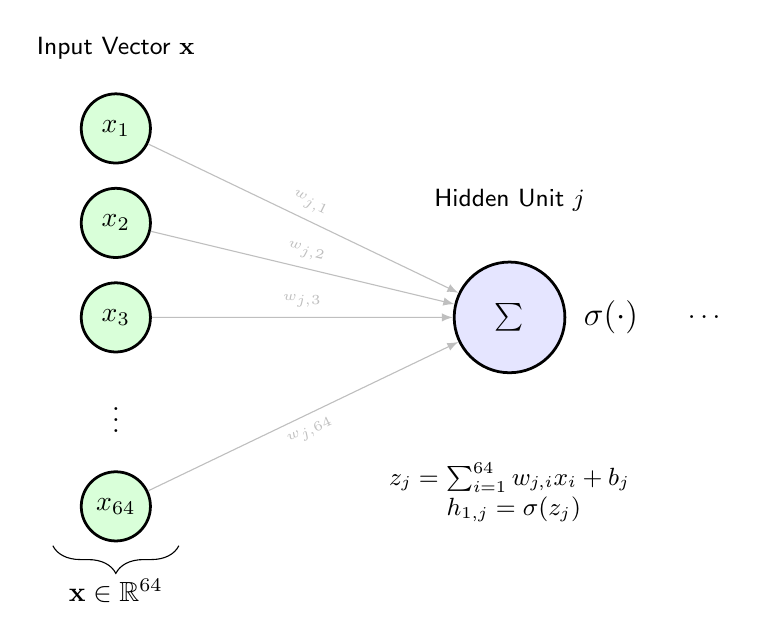
\begin{tikzpicture}[
    neuron/.style={circle, draw, minimum size=25pt, inner sep=0pt, line width=1pt},
    input/.style={neuron, fill=green!15},
    hidden/.style={neuron, fill=blue!10},
    connect/.style={-latex, thin, gray!50},
    label_style/.style={font=\small\sffamily}
]

    % --- DRAW INPUT LAYER ---
    \foreach \i in {1,2,3} {
        \node[input] (I-\i) at (0, -\i*1.2) {$x_{\i}$};
    }
    \node at (0, -4.8) {$\vdots$};
    \node[input] (I-n) at (0, -6) {$x_{64}$};
    
    \node[above=0.3cm of I-1, label_style] {Input Vector $\mathbf{x}$};

    % --- DRAW SINGLE HIDDEN NEURON ---
    % We place one large neuron representing the j-th unit
    \node[hidden, minimum size=40pt] (H1) at (5, -3.6) {$\sum$};
    \node[right=0.1cm of H1, font=\large] (act) {$\sigma(\cdot)$};
    
    \node[above=0.5cm of H1, label_style] {Hidden Unit $j$};

    % --- DRAW CONNECTIONS WITH LABELS ---
    \draw[connect] (I-1) -- (H1) node[midway, above, sloped, font=\tiny] {$w_{j,1}$};
    \draw[connect] (I-2) -- (H1) node[midway, above, sloped, font=\tiny] {$w_{j,2}$};
    \draw[connect] (I-3) -- (H1) node[midway, above, sloped, font=\tiny] {$w_{j,3}$};
    \draw[connect] (I-n) -- (H1) node[midway, below, sloped, font=\tiny] {$w_{j,64}$};

    % --- ADD THE MATRIX MATH ---
    % Summation label
    \node[below=1cm of H1, align=center, font=\small] (math) {
        $z_j = \sum_{i=1}^{64} w_{j,i} x_i + b_j$ \\
        \vspace{0.2cm}
        $h_{1,j} = \sigma(z_j)$
    };

    % Braces for Matrix Representation
    \draw [decorate, decoration={brace, amplitude=10pt, mirror}] 
        (-0.8,-6.5) -- (0.8,-6.5) node [black, midway, below=0.3cm] {$\mathbf{x} \in \mathbb{R}^{64}$};

    \node at (7.5, -3.6) {$\dots$};

\end{tikzpicture}
\end{document}